%!TEX root = iclr2026_conference.tex
% Appendix F (sec:app:development): F.1 development and in-sample diagnostics of the submitted checkpoint, F.2 the
% identity-disjoint evaluation-split rerun, F.3 submitted-model facts, the withdrawn compute record and implementation
% details. Content plan and owner unit: manuscript/paper-contract.md §8 (W3). F.3 holds the moved CLEVRER Replication
% Details and Implementation Details as subsubsections; their labels sec:app:clevrer and sec:app:impl are kept.
% Number anchors (relative to NovPhy/): S1 = .local-artifacts/issue-96-tau-ad-within-checkpoint-v1/summary.json;
% rerun = .local-artifacts/issue-104-heldout-contrasts-v1/{summary.json,findings.md}; LOSO =
% .local-artifacts/issue-117-item5-benchmarks-v1/findings.md; compute correction =
% .local-artifacts/issue-103-engine-truth-frontier-v1/compute.json .iclr_sentence; parser = docs/issue-99-*.md §1-2.
\section{\texorpdfstring{\rev{Submitted-Checkpoint Evidence}}{Submitted-Checkpoint Evidence}}
\label{sec:app:development}

\begin{revblock}
The submitted comparisons mixed changes in predictor training, request execution, and learned selection; these are distinct sources of performance differences. We retain the submitted records as historical evidence and use the revised same-checkpoint controls to distinguish trained-policy differences from inference-time request restrictions. Those controls are reported in Section~\ref{sec:res:ranking} and Appendix~\ref{sec:app:results}.

This appendix keeps the evidence of the submitted checkpoint and states what each record shows and what it does not show. Section~\ref{sec:app:dev:insample} collects the submitted development and in-sample diagnostics. Every submitted record there was measured on scenes, trials or levels used during model development, so none of them is evidence of generalization. It also contains one post-submission exploratory refit, labelled as such. Section~\ref{sec:app:dev:rerun} reruns the submitted checkpoint on the 400-level evaluation split of Section~\ref{sec:mth:protocol}. That rerun is not in-sample, and we keep it separate from the development records. Section~\ref{sec:app:dev:model} gives the submitted model's facts and implementation, and the withdrawn compute comparison together with its correction, which is a post-submission evaluation-split record of the primary predictors.

One fact governs how the ranking records below can be read. The submitted frozen parser detected the pig in 0 of 859 decision frames of the development-inventory shots, so the pig term of the submitted count cost carried no information on those records (Section~\ref{sec:app:dev:facts}).

\textbf{Submitted checkpoint.} The submitted checkpoint is the hybrid predictor, the continuous predictor and the request policies trained on them, as submitted, with model seeds 20260908, 20260909 and 20260910. It differs from the primary model of Section~\ref{sec:mth:model} in three ways. Its encoder is the earlier frozen parser, its training data mix two time bases, and it was trained with the short-window recipe, without the long-horizon and decision-contrastive losses (Section~\ref{sec:app:dev:facts}).

\textbf{Notation.} Inside this appendix we keep the submitted names where a record uses them, mapped once to the revised notation. The submission's fixed-request reference $r^\dagger$, also called the ``transferred fixed request'' or the ``fixed request tuned on the other three sets'', is $F^{*}$: the fixed request with the best mean ordering AUC (Equation~\ref{eq:auc}) on the other three inventories. Its ``hybrid adaptive'' policy is $J$ of the submitted checkpoint, not the retrained $J$ of Section~\ref{sec:mth:model}. Its ``horizon-only adaptive baseline'' is $C\text{-}J$ on the submitted continuous predictor, and its ``launch set'' is an inventory. $F_{\mathrm{hind}}$ is the best fixed request on the scored inventory in hindsight. Records of this appendix score candidates either by the submitted \emph{count cost} (Equation~\ref{eq:select}), which reads clipped pig and block presences on the predicted carrier at $t=225$, or by the \emph{tie-free cost} (Equation~\ref{eq:taskcost}), pig presence minus $0.1$ times the pig-centre displacement from the decision-frame carrier. Each table and figure names its cost. Because clipped presences saturate, the count cost can assign the same value to every candidate of a cell. Such a cell is \emph{fully tied}, and its ordering AUC is 0.5.
\end{revblock}

\subsection{\texorpdfstring{\rev{Development and In-Sample Diagnostics of the Submitted Checkpoint}}{Development and In-Sample Diagnostics of the Submitted Checkpoint}}
\label{sec:app:dev:insample}

\begin{revblock}
This subsection reproduces the submitted diagnostics and relabels each one. The rollout-error table measures longer rollouts on fitting scenes (CLEVRER, Physion-Dominoes) and on development levels (NovPhy) (Section~\ref{sec:app:dev:rollout}). The heatmap and the per-inventory records describe ordering AUC on four small development inventories (Sections~\ref{sec:app:dev:grid} and~\ref{sec:app:dev:s1}). The qualitative figure shows one decision (Section~\ref{sec:app:dev:qual}). Section~\ref{sec:app:dev:model} gives the model facts needed to read these records.
\end{revblock}

\subsubsection{\texorpdfstring{\rev{Rollout Error on Annotation Carriers}}{Rollout Error on Annotation Carriers}}
\label{sec:app:dev:rollout}

\begin{table}[t]
\centering
\small
\begin{revblock}
\caption{\textbf{Submitted rollout-error table (development, in-sample diagnostic of the submitted checkpoint).} Mean squared error of the predicted object positions at the last endpoint, 225 carrier frames on NovPhy and 120 frames on CLEVRER and Physion-Dominoes, rolled recursively from one observed carrier (three-seed mean, as submitted). CLEVRER and Physion-Dominoes carriers were built from released object annotations. CLEVRER fitting windows and evaluation rollouts came from the same 12 scenes (10000--10011), and Physion-Dominoes used 12 trials from within one release. On these two benchmarks the table therefore measures longer rollouts on fitting scenes, not scene generalization. NovPhy rollouts started from 4 N1 levels held out from fitting but used as development diagnostics, with 13 launches each. The very large $\Delta=1$ errors are consistent with the short-window training recipe: long-horizon supervision removes the $\Delta=1$ divergence on NovPhy (Section~\ref{sec:res:rollout}) and, in the exploratory refit of Section~\ref{sec:app:dev:rollout}, on CLEVRER and Physion-Dominoes. Baseline: the submitted continuous-only predictor. Hybrid: the submitted predictor serving all nine requests. No macro arm was trained on CLEVRER or Physion-Dominoes (--).}
\label{tab:app:dev:rollout}
\end{revblock}
\begin{tabular}{@{}llrrr@{}}
\toprule
Model & Request $r$ & NovPhy & CLEVRER & Physion-Dominoes \\
\midrule
Baseline & $(1,\textsf{cont})$  & 2224   & 13.5   & 182.6 \\
         & $(5,\textsf{cont})$  & 0.281  & 0.0471 & 0.0176 \\
         & $(15,\textsf{cont})$ & 0.0370 & 0.0116 & 0.00114 \\
\midrule
Hybrid   & $(1,\textsf{cont})$  & 3141   & 2.98   & 167.4 \\
         & $(5,\textsf{cont})$  & 0.200  & 0.0444 & 0.0156 \\
         & $(15,\textsf{cont})$ & 0.0296 & 0.0170 & 0.00128 \\
         & $(15,\textsf{micro})$ & 0.0313 & 0.0190 & 0.00199 \\
         & $(15,\textsf{macro})$ & 0.0397 & --     & -- \\
\bottomrule
\end{tabular}
\end{table}

\begin{revblock}
Table~\ref{tab:app:dev:rollout} shows that, on development scenes and levels and under the short-window recipe, rollouts that advance 15 frames per prediction end with far lower position error than rollouts that advance one frame. It does not show scene generalization, and it does not show a recipe-independent ordering. The held-out evidence for rollout error is the sealed NovPhy grid and the separate pixel-carrier study of Section~\ref{sec:res:rollout}.

\textbf{Exploratory leave-one-scene-out refit (post-submission).} After submission we refit on the original 12 scenes in twelve folds, each holding out one scene, and scored rollouts on the held-out scene, with three seeds per fold (\#117 item 5). The folds use six requests, $\Delta\in\{1,5,15\}\times\{\textsf{cont},\textsf{micro}\}$, and no macro arm, so they do not replace the table. Under the submitted recipe the coarse-horizon ordering persists on held-out scenes. At $t=120$ the shared predictor's position error is 16.277 [9.097, 26.428] for $(1,\textsf{cont})$ and 0.091 [0.060, 0.128] for $(15,\textsf{cont})$ on CLEVRER, and 360.487 [292.485, 436.284] against 0.003 [0.002, 0.006] on Physion-Dominoes (mean over held-out scenes, scene-clustered 95\% intervals). Under the long-horizon recipe the $(1,\textsf{cont})$ error falls to 0.081 [0.059, 0.104] on CLEVRER and 0.013 [0.004, 0.028] on Physion-Dominoes, against 0.067 [0.047, 0.091] and 0.008 [0.002, 0.018] for $(15,\textsf{cont})$. The refit is exploratory: twelve held-out scenes are a small sample, and the folds reuse the scene pool and annotation carriers of the original experiment.
\end{revblock}

\subsubsection{\texorpdfstring{\rev{Fixed-Request Ordering AUC on the Development Inventories}}{Fixed-Request Ordering AUC on the Development Inventories}}
\label{sec:app:dev:grid}

\begin{figure}[t]
\centering
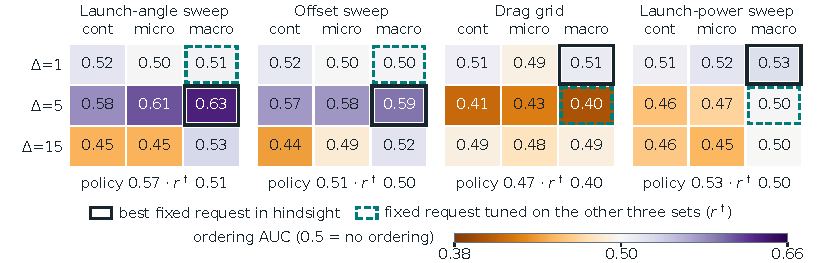
\includegraphics[width=\linewidth]{figures/fig_results_grid.pdf}
\begin{revblock}
\caption{\textbf{Fixed-request ordering AUC on the development launch inventories (submitted checkpoint, count cost, development diagnostic).} Each cell is the mean ordering AUC of one fixed request $F(\Delta,\alpha)$ of the submitted hybrid over the mixed-outcome levels and three seeds of one inventory. A value of 0.5 is chance ordering, and the 36 cell means lie between 0.40 and 0.63. Panels: launch-angle sweep (angle), offset sweep (offset), drag grid (grid), launch-power sweep (power). The four inventories are drawn from the same 15 exposed development levels and contain 14 (grid), 9 (offset), 7 (angle) and 8 (power) mixed levels. Solid box: $F_{\mathrm{hind}}$. Dashed box: $F^{*}$, chosen by mean AUC on the other three inventories over the same levels (labelled $r^\dagger$ in the artwork). Below each panel: the AUC of $J$ (``policy'') and of $F^{*}$. Per-cell intervals are in Table~\ref{tab:app:dev:s1arms}. The submitted per-inventory reading of this figure is descriptive.}
\label{fig:app:dev:grid}
\end{revblock}
\end{figure}

\begin{revblock}
Figure~\ref{fig:app:dev:grid} is the submitted heatmap. The submission read it per inventory: $(5,\textsf{macro})$ ranked first on angle and offset and last on grid, and the best fixed request used $\textsf{macro}$ on every inventory. Those readings rest on 7--14 mixed levels per inventory, and the intervals are wide. For example, grid $F(15,\textsf{cont})$ scores 0.492 [0.411, 0.584] (Table~\ref{tab:app:dev:s1arms}). The figure shows that fixed-request AUCs on these development levels lie near chance and that their order changes between inventories. It does not establish which request is best on new levels. The description-mode reading is narrowed in Section~\ref{sec:res:ranking}.
\end{revblock}

\subsubsection{\texorpdfstring{\rev{Numerical Supplement S1: Development-Inventory Records}}{Numerical Supplement S1: Development-Inventory Records}}
\label{sec:app:dev:s1}

\begin{table}[t]
\centering
\scriptsize
\setlength{\tabcolsep}{2pt}
\begin{revblock}
\caption{\textbf{Supplement S1, per inventory (submitted checkpoint, development inventories, count cost).} Eligible: levels with a complete inventory (angle has 14 because one level was excluded as unmeasurable before scoring). Mixed: levels whose inventory holds both a success and a failure, shown as mixed levels / cells, with cells $=$ mixed levels $\times$ 3 seeds. Slots: distinct successful candidates over the mixed levels, not choices by $J$ and not multiplied by seed, shown with the number of those successes that the engine resolves by carrier frame 225. $F^{*}$: the fixed request with the best mean ordering AUC on the other three inventories ($=r^\dagger$ of the submission). $J-F^{*}$: paired ordering-AUC difference with its descriptive 95\% level-clustered percentile bootstrap interval (10{,}000 draws). HW: its half-width. Top-1: cells in which the first-ranked candidate succeeds, shown as $J$ / $F^{*}$.}
\label{tab:app:dev:s1}
\begin{tabular}{@{}lrrrllrr@{}}
\toprule
Inventory & Eligible & Mixed & Slots & $F^{*}$ & $J-F^{*}$ [95\% CI] & HW & Top-1 \\
\midrule
Grid   & 15 & 14 / 42 & 17 / 11 & $F(5,\textsf{macro})$ & $+0.0700$ [$-0.0057$, $+0.1437$] & 0.0747 & 0/42 / 0/42 \\
Offset & 15 & 9 / 27  & 9 / 3   & $F(1,\textsf{macro})$ & $+0.0037$ [$-0.0796$, $+0.0926$] & 0.0861 & 0/27 / 1/27 \\
Angle  & 14 & 7 / 21  & 7 / 5   & $F(1,\textsf{macro})$ & $+0.0595$ [$+0.0079$, $+0.1131$] & 0.0526 & 0/21 / 0/21 \\
Power  & 15 & 8 / 24  & 8 / 4   & $F(5,\textsf{macro})$ & $+0.0273$ [$-0.0691$, $+0.1281$] & 0.0986 & 0/24 / 0/24 \\
\bottomrule
\end{tabular}
\end{revblock}
\end{table}

\begin{table}[t]
\centering
\footnotesize
\setlength{\tabcolsep}{4pt}
\begin{revblock}
\caption{\textbf{Supplement S1, every retained arm (submitted checkpoint, development inventories, count cost).} Mean ordering AUC [95\% level-clustered interval] over the mixed cells of each inventory (0.5 is chance). $F(\Delta,\alpha)$: fixed request on the submitted hybrid. $J$: the submitted request policy. $T$ and $D$: $J$ restricted to its modal description (adapts $\Delta$ only) or to its modal horizon (adapts $\alpha$ only), with modal coordinates taken per seed from $J$'s request frequencies. $M$: factorized selector that chooses $\Delta$ and $\alpha$ separately from $J$'s logits, without training. $OL$: open-loop schedule drawn i.i.d.\ from $J$'s pooled request frequencies, independent of the imagined state. $C\text{-}F(\Delta)$ and $C\text{-}J$: fixed continuous requests and the horizon-only policy on the submitted continuous predictor. These controls differ from the same-checkpoint $J_{\mathrm{cont}}^{\mathrm{NovPhy}}$ of Section~\ref{sec:res:ranking}.}
\label{tab:app:dev:s1arms}
\begin{tabular}{@{}lllll@{}}
\toprule
Arm & Grid & Offset & Angle & Power \\
\midrule
$F(1,\textsf{cont})$   & 0.510 [0.483, 0.536] & 0.517 [0.481, 0.556] & 0.520 [0.500, 0.544] & 0.509 [0.488, 0.536] \\
$F(1,\textsf{micro})$  & 0.493 [0.464, 0.520] & 0.500 [0.489, 0.511] & 0.502 [0.446, 0.560] & 0.520 [0.504, 0.542] \\
$F(1,\textsf{macro})$  & 0.513 [0.467, 0.563] & 0.504 [0.444, 0.559] & 0.506 [0.423, 0.583] & 0.527 [0.474, 0.592] \\
$F(5,\textsf{cont})$   & 0.415 [0.337, 0.480] & 0.574 [0.507, 0.648] & 0.581 [0.497, 0.663] & 0.458 [0.374, 0.549] \\
$F(5,\textsf{micro})$  & 0.425 [0.368, 0.484] & 0.576 [0.491, 0.659] & 0.609 [0.554, 0.671] & 0.469 [0.379, 0.546] \\
$F(5,\textsf{macro})$  & 0.401 [0.348, 0.461] & 0.594 [0.517, 0.674] & 0.635 [0.587, 0.679] & 0.501 [0.414, 0.606] \\
$F(15,\textsf{cont})$  & 0.492 [0.411, 0.584] & 0.441 [0.348, 0.504] & 0.450 [0.323, 0.561] & 0.462 [0.403, 0.528] \\
$F(15,\textsf{micro})$ & 0.479 [0.395, 0.578] & 0.487 [0.415, 0.544] & 0.450 [0.359, 0.524] & 0.452 [0.399, 0.520] \\
$F(15,\textsf{macro})$ & 0.491 [0.455, 0.526] & 0.522 [0.489, 0.559] & 0.534 [0.500, 0.569] & 0.499 [0.438, 0.559] \\
\midrule
$J$  & 0.471 [0.416, 0.526] & 0.507 [0.456, 0.559] & 0.565 [0.520, 0.625] & 0.529 [0.469, 0.591] \\
$T$  & 0.498 [0.463, 0.530] & 0.541 [0.507, 0.581] & 0.553 [0.525, 0.579] & 0.523 [0.475, 0.572] \\
$D$  & 0.509 [0.459, 0.568] & 0.530 [0.452, 0.607] & 0.486 [0.389, 0.569] & 0.509 [0.466, 0.556] \\
$M$  & 0.492 [0.435, 0.546] & 0.524 [0.480, 0.574] & 0.571 [0.521, 0.631] & 0.550 [0.507, 0.591] \\
$OL$ & 0.523 [0.474, 0.574] & 0.509 [0.474, 0.544] & 0.543 [0.508, 0.579] & 0.537 [0.483, 0.588] \\
\midrule
$C\text{-}F(1)$  & 0.468 [0.447, 0.487] & 0.520 [0.489, 0.552] & 0.477 [0.433, 0.526] & 0.509 [0.474, 0.550] \\
$C\text{-}F(5)$  & 0.486 [0.432, 0.533] & 0.624 [0.528, 0.709] & 0.576 [0.508, 0.650] & 0.605 [0.491, 0.728] \\
$C\text{-}F(15)$ & 0.506 [0.430, 0.586] & 0.552 [0.459, 0.641] & 0.475 [0.405, 0.544] & 0.577 [0.495, 0.677] \\
$C\text{-}J$     & 0.522 [0.474, 0.566] & 0.546 [0.496, 0.593] & 0.546 [0.488, 0.611] & 0.558 [0.497, 0.606] \\
\bottomrule
\end{tabular}
\end{revblock}
\end{table}

\begin{revblock}
Tables~\ref{tab:app:dev:s1} and~\ref{tab:app:dev:s1arms} give the complete retained record behind the submitted claim that $J$ ranks launches better than $F^{*}$ on every inventory. Only the angle interval for $J-F^{*}$ excludes zero. The grid contrast was the pre-declared primary, and two of its guards failed: 17 of 42 cells had $J$ or $F^{*}$ fully tied (share 0.405, against a maximum of 0.20), and the half-width was 0.0747 (against a maximum of 0.05). The primary reading is therefore precision-insufficient. $J$'s first-ranked candidate never succeeded, in 0/42, 0/27, 0/21 and 0/24 cells, and $F^{*}$'s succeeded once (offset, 1/27).

$F^{*}$ is a cross-inventory choice. It is selected with outcomes from the other three inventories, and all four inventories cover the same 15 levels, so $F^{*}$ is not member-disjoint and its intervals are selection-conditional. It is neither a hindsight-best nor an independently selected reference.
\end{revblock}

\subsubsection{\texorpdfstring{\rev{One Decision on One Development Level}}{One Decision on One Development Level}}
\label{sec:app:dev:qual}

\begin{figure}[t]
\centering
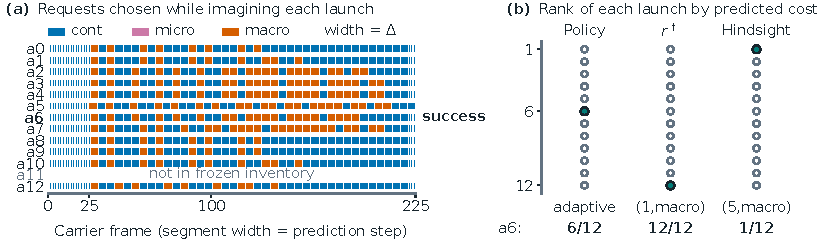
\includegraphics[width=\linewidth]{figures/fig_qualitative_requests.pdf}
\begin{revblock}
\caption{\textbf{One decision on one development level (submitted checkpoint, count cost).} Angle inventory of the level shown in Figure~\ref{fig:levels}, model seed 20260908. The 12 candidate launches run from flat (a0) to steep (a12). Launch a11 is not in the frozen inventory, and only a6 succeeds in the engine. (a) Requests $J$ chooses while imagining each launch to carrier frame 225. Each segment is one prediction, coloured by $\alpha$, with width $\Delta$. (b) Rank of each launch by predicted count cost (1 = chosen) under $J$ (``adaptive''), under $F^{*}=(1,\textsf{macro})$ (labelled $r^\dagger$) and under $F_{\mathrm{hind}}=(5,\textsf{macro})$. The filled dot is a6. This is one decision, not a frequency estimate.}
\label{fig:app:dev:qual}
\end{revblock}
\end{figure}

Figure~\ref{fig:app:dev:qual} opens one decision. While imagining each launch, the policy starts with single-frame steps and then alternates $(5,\textsf{cont})$ and $(5,\textsf{macro})$, and where it places the $\textsf{macro}$ steps depends on the launch: the 12 candidates receive eight different schedules. \rev{On this decision, the resulting order sits between the two fixed references.} The policy ranks the one successful launch, a6, sixth of 12, the transferred fixed request $(1,\textsf{macro})$ ranks it last, and the best fixed request in hindsight, $(5,\textsf{macro})$, ranks it first. \rev{Across all 2,634 imagined rollouts of the development inventories, the schedule differs between candidate launches in 77\% of level--seed pairs.} Longer and coarser requests become more frequent as the rollout proceeds: the share of $\Delta=5$ rises from 2\% of predictions in the first 25 frames to 16\% after frame 100, and the share of $\textsf{macro}$ from 59\% to 83\%.

\begin{revblock}
These schedule statistics describe the submitted $J$ on development levels. They show that its schedule varies with the imagined launch. They do not establish that this variation improves ranking. On the development grid records, replacing $J$'s choices by open-loop draws from its own request frequencies gives $J-OL=-0.0520$ [$-0.1192$, $+0.0173$]. On the evaluation-split rerun (tie-free cost, Section~\ref{sec:app:dev:rerun}) the same contrast is $J-OL=+0.0401$ [$+0.0247$, $+0.0556$]. That rerun reading is precision-insufficient because the rerun's grid precision guard failed. $J-OL$ compares $J$ with its own open-loop schedule, not with a fixed request, and does not bear on the withdrawn claim.
\end{revblock}

\subsection{\texorpdfstring{\rev{Identity-Disjoint Rerun of the Submitted Checkpoint on the Evaluation Split}}{Identity-Disjoint Rerun of the Submitted Checkpoint on the Evaluation Split}}
\label{sec:app:dev:rerun}

\begin{table}[t]
\centering
\scriptsize
\setlength{\tabcolsep}{2pt}
\begin{revblock}
\caption{\textbf{Submitted checkpoint rerun on the identity-disjoint evaluation split (endpoint $t=225$, three seeds).} Mixed levels hold both engine outcomes, with cells $=$ mixed levels $\times$ 3 seeds. $F^{*}$: the fixed request with the best mean ordering AUC on the other three inventories ($=r^\dagger$ of the submission), re-selected on this split under each cost. Under the count cost it is $F(5,\textsf{macro})$ on every inventory. $J-F^{*}$: paired ordering-AUC difference with its descriptive 95\% level-clustered percentile bootstrap interval (10{,}000 draws). HW: its half-width. AUC columns give mean ordering AUC under the tie-free cost (0.5 is chance). Under each cost the frozen guards fail: the tie-free grid half-width exceeds its limit of 0.02, and the count cost fails its own tie and precision guards. Every contrast is therefore precision-insufficient. Inventories are never pooled, and the non-grid inventories use 120 of the 400 levels.}
\label{tab:app:dev:rerun}
\begin{tabular}{@{}lrlllrrl@{}}
\toprule
 & & \multicolumn{5}{c}{Tie-free cost (primary)} & Count cost (secondary) \\
\cmidrule(lr){3-7}\cmidrule(l){8-8}
Inventory & Mixed (cells) & $F^{*}$ & $J-F^{*}$ [95\% CI] & HW & AUC $J$ & AUC $F^{*}$ & $J-F^{*}$ [95\% CI] \\
\midrule
Grid   & 311 (933) & $F(5,\textsf{macro})$ & $+0.0134$ [$-0.0163$, $+0.0431$] & 0.0297 & 0.555 & 0.542 & $+0.0893$ [$+0.0685$, $+0.1107$] \\
Offset & 76 (228)  & $F(5,\textsf{cont})$  & $+0.0111$ [$-0.0520$, $+0.0743$] & 0.0632 & 0.410 & 0.399 & $-0.1152$ [$-0.1559$, $-0.0762$] \\
Angle  & 78 (234)  & $F(5,\textsf{macro})$ & $-0.1596$ [$-0.2061$, $-0.1130$] & 0.0466 & 0.439 & 0.599 & $-0.0874$ [$-0.1243$, $-0.0518$] \\
Power  & 47 (141)  & $F(5,\textsf{macro})$ & $-0.2617$ [$-0.3360$, $-0.1921$] & 0.0720 & 0.459 & 0.721 & $-0.0323$ [$-0.0830$, $+0.0177$] \\
\bottomrule
\end{tabular}
\end{revblock}
\end{table}

\begin{revblock}
On the identity-disjoint evaluation split, the submitted conclusion that $J$ ranks launches better than a cross-inventory fixed request does not survive under either cost (Table~\ref{tab:app:dev:rerun}). The rerun applied the submitted predictors and request policies, unchanged, to the 400 evaluation levels of Section~\ref{sec:mth:protocol} and scored the contrast set of Supplement S1 under a plan frozen before any score of this rerun existed (\#104). Every candidate is imagined to $t=225$ from its level's decision-frame carrier, parsed by the submitted checkpoint's parser (Section~\ref{sec:app:dev:facts}). Outcomes are the recorded engine verdicts. The pre-declared primary cost is the tie-free cost, and the submitted count cost is a secondary reading. No level of this split was used to fit or train the submitted models, so the rerun is not in-sample. The split is identity-disjoint but within-distribution (Section~\ref{sec:mth:protocol}).

Evaluation outcomes are excluded from fitting the predictors, training the policies, and choosing their deployment hyperparameters. Explicitly labelled hindsight comparisons, cross-inventory reference choices, and observed-frontier summaries use evaluation outcomes and are not independently selected deployment policies. In this rerun, $F^{*}$ and $F_{\mathrm{hind}}$ are such choices.

Under the tie-free cost, the grid contrast is $J-F^{*}=+0.0134$ [$-0.0163$, $+0.0431$]. The frozen precision guard requires the grid half-width to be at most 0.02. The rerun plan tightened the development plan's bound of 0.05 (Section~\ref{sec:app:dev:s1}) to this value. The observed half-width is 0.0297, so the guard fails and every token of the rerun is precision-insufficient. The non-grid half-widths, 0.0632, 0.0466 and 0.0720, also exceed 0.02. Offset is inconclusive, at $+0.0111$ [$-0.0520$, $+0.0743$]. On angle and power, $J$'s AUC is descriptively lower than $F^{*}$'s, by $-0.1596$ [$-0.2061$, $-0.1130$] and $-0.2617$ [$-0.3360$, $-0.1921$], and both intervals exclude zero. None of the three non-grid inventories replicates a positive contrast (0 of 3 have a mean of at least $\delta$ with a lower bound above zero).

The submitted count cost does not reverse this reading. Its grid contrast is positive, $J-F^{*}=+0.0893$ [$+0.0685$, $+0.1107$], but 395 of 933 cells have $J$ or $F^{*}$ fully tied (share 0.42, against a maximum of 0.20). Its half-width is 0.0211, so both its tie guard and its precision guard fail. On the other inventories the count-cost contrasts are $-0.1152$ [$-0.1559$, $-0.0762$] (offset), $-0.0874$ [$-0.1243$, $-0.0518$] (angle) and $-0.0323$ [$-0.0830$, $+0.0177$] (power). Under both costs, $J$ does not rank launches better than $F^{*}$ on any non-grid inventory.

On the grid under the tie-free cost, $J$ scores 0.555 [0.539, 0.571] and $F^{*}$ 0.542 [0.520, 0.564]. The hindsight-best fixed request, $F_{\mathrm{hind}}=F(15,\textsf{cont})$, scores 0.639, and $J-F_{\mathrm{hind}}=-0.0841$ [$-0.1147$, $-0.0537$]. The other grid contrasts of the set are $J-M=+0.0080$ [$-0.0044$, $+0.0204$], $J-T=-0.0011$ [$-0.0145$, $+0.0128$], $J-D=+0.0582$ [$+0.0368$, $+0.0794$] and $J-OL=+0.0401$ [$+0.0247$, $+0.0556$], with $M$, $T$, $D$ and $OL$ defined as in Table~\ref{tab:app:dev:s1arms}. All four are precision-insufficient because the grid guard failed.

The original adaptivity conclusion therefore does not survive on new levels under either cost. The submission's offset gain of about $+0.004$ (Table~\ref{tab:app:dev:s1}: $+0.0037$ [$-0.0796$, $+0.0926$], against $F^{*}=F(1,\textsf{macro})$) is not a replicated effect. The rerun estimate is $+0.0111$ [$-0.0520$, $+0.0743$] with a failed precision guard, against $F^{*}=F(5,\textsf{cont})$. Because $F^{*}$ is re-selected on the evaluation split by the same rule, the two offset estimates compare $J$ with different fixed requests. Section~\ref{sec:res:ranking} reports the same rerun in the main text.
\end{revblock}

\subsection{\texorpdfstring{\rev{Submitted Model Facts, Withdrawn Compute Record and Implementation}}{Submitted Model Facts, Withdrawn Compute Record and Implementation}}
\label{sec:app:dev:model}

\begin{revblock}
This subsection gives the facts about the submitted model that the records of Sections~\ref{sec:app:dev:insample} and~\ref{sec:app:dev:rerun} depend on, the withdrawn compute comparison with its correction, and the moved implementation details.
\end{revblock}

\subsubsection{\texorpdfstring{\rev{Submitted Model Facts}}{Submitted Model Facts}}
\label{sec:app:dev:facts}

\begin{revblock}
\textbf{Training data and time base.} The submitted predictors were fit on 2,409 lineages, where a lineage is a generated scene identity together with the launches and windows derived from it. Of these, 2,400 belong to the \emph{base corpus}, the earlier collection of 3,000 training-role NovPhy lineages (2,400 for predictor fitting and 600 for policy supervision). The other 9 are \emph{N1} lineages. N1 captures are the later normal-condition campaigns that record one carrier frame every 50 native engine steps (0.02\,s). The policies were supervised on 603 lineages, the 600 base-corpus policy lineages and 3 N1 lineages. In the base corpus, $\Delta$ counted native fixed-step frames inside 60-step windows, and the physical duration of one such step was not verified. On N1, $\Delta=1/5/15$ spans 50/250/750 native steps. The same request code therefore denotes a 50 times longer native-step interval on N1 than in the base corpus. The carrier's elapsed-seconds entry makes the cadence available, but no elapsed-channel ablation was run. We therefore do not claim that the submitted model reconciled the two rates, and we make no cross-time-base transfer claim. The development inventories of Section~\ref{sec:app:dev:s1} and the evaluation split of Section~\ref{sec:app:dev:rerun} are both captured at the 50-step N1 stride.

\textbf{Perception.} The submitted frozen parser read the pig as present in 0 of 859 decision frames of the retained development-inventory shots, although the engine had the pig in all 859. At the endpoint it read the pig in 10 of 859 frames (engine: 836). The pig term of the count cost was therefore uninformative on these records. The repaired encoder of the primary model reads the pig at the start of all 240 held-out development shots (accuracy 1.000).
\end{revblock}

\subsubsection{\texorpdfstring{\rev{Withdrawn Compute Comparison}}{Withdrawn Compute Comparison}}
\label{sec:app:dev:compute}

\begin{revblock}
\textbf{Submitted sentence (withdrawn).} The submission stated that choosing both axes ``matches a horizon-only adaptive baseline at a third of its compute''. The evidence was a comparison on 200 development states with 12 candidate launches each. $J$'s regret was 0.350 against 0.367 for $C\text{-}J$, at 118.7M against 356.0M multiply-accumulates per candidate and state, and 1.0\,s against 2.0\,s of wall time per state.

\textbf{Why it is withdrawn.} Four properties of that comparison prevent it from supporting the sentence. (i)~The regret was a proxy, computed from the count cost and normalized per state to $[0,1]$, not from task success. (ii)~Both models came from a different training, an earlier run of the same recipe on the 2,400 base-corpus lineages alone (Section~\ref{sec:app:impl}). (iii)~The 200 states were exposed development states, not evaluation levels. (iv)~The two predictors have trunks of different widths, 456 for the continuous predictor against 384 for the hybrid, so the multiply-accumulate difference mixes trunk width with request selection.

\textbf{Correction (post-submission, evaluation split, primary predictors).} An engine-truth re-evaluation repeats the comparison on the sealed grid (311 mixed levels $\times$ 3 seeds) with the $J$ and $C\text{-}J$ of Section~\ref{sec:mth:model}, which apply the submitted policy recipe ($\lambda=10^{-4}$) to the revised predictors. Counting linear MACs of predictor and policy calls per candidate rollout to $t=225$, with nonlinear and memory work excluded, $J$ costs 184.0M and $C\text{-}J$ 234.7M, a ratio of 0.784 rather than one third. The AUC difference is $J-(C\text{-}J)=+0.006$ [$0.000$, $+0.012$], below the practical margin $\delta=0.02$. The saving comes primarily from the narrower predictor trunk, and description modes add cost (Section~\ref{sec:res:compute}). No wall-time speedup for $J$ was observed. $J$'s wall time per state is 16.74 times that of $C\text{-}J$ in the frozen single-seed timing and 1.63 times in a post-hoc three-seed retiming.
\end{revblock}

\subsubsection{CLEVRER Replication Details}
\label{sec:app:clevrer}

This \rev{subsection} documents the CLEVRER replication: data provenance, frozen membership rule, Phase-0 vocabulary mapping, endpoint grid, and training protocol.
The data source is the official CLEVRER release at \texttt{data.csail.mit.edu/\allowbreak clevrer} under a CC0 license \citep{yi2020clevrer}. Only the annotation archives were used: train at 156{,}761{,}889 bytes with \texttt{sha256} prefix \texttt{e7f9185a} and validation at 78{,}386{,}966 bytes with prefix \texttt{d89e7471}. No videos were downloaded. Train scenes 0--9999 and validation scenes 10000--14999 ship annotations, and the test split ships none. Each annotation contains \texttt{object\_property} records for color, material, and shape, per-frame \texttt{motion\_trajectory} entries with per-object location, orientation, velocity, and angular velocity, collision events with \texttt{frame\_id}, and an \texttt{inside\_camera\_view} flag. That flag is the availability mask, applied in slot columns 7 and 10 and in every masked estimand, and unavailable fields are zeroed exactly as the deployment carrier zeroes them. Vertical location and velocity, orientation matrices, and angular velocities are parsed into per-scene shards for the parser-contract record with no carrier-column referent. No official generation or simulation code exists. The public CLEVRER repository at pinned commit \texttt{98b8420} contains model code only, and the paper's Bullet-plus-Blender pipeline was never released, so regenerated scenes are not a fallback. Had the released fields proved insufficient for the feature-parser contract, the frozen rule required publishing \texttt{readiness\_or\_precision\_\allowbreak insufficient} naming the exact blocker.

Membership was frozen before any training. The rule selects the first 12 collision-complete scenes in ascending \texttt{scene\_index} within the validation-split annotations, where collision-complete means a contiguous 128-frame trajectory for every declared object and at least one collision event, with no outcome-based selection. The selected scenes are 10000 through 10011, with 4 to 6 objects and 1 to 4 collisions each. Each scene yields 40 training windows with starts 0 through 39 and length 61, for 480 windows in total, and the evaluation contexts $\{0,1,2,3\}$ give 48 scene--context units per seed. The scan visited exactly these 12 scenes and skipped none, and the membership function returns typed failures for skipped scenes rather than dropping them silently. \rev{Training windows and evaluation contexts therefore come from the same 12 scenes, and the CLEVRER errors of Table~\ref{tab:app:dev:rollout} are in-sample.}

The Phase 0 vocabulary mapping was declared before any training. The carrier reuses the unchanged \#71 layout of 2 global values plus 18 slots of 13 columns, with kind vocabulary cube, cylinder, and sphere, position scale 5.0, velocity scale 3.0, and speed-tier edges frozen at $[0.3499, 1.6807]$. The micro predicates are contact, derived from collision events as symmetric channel 0, and velocity-bin, a same-tier indicator at the frozen edges as symmetric channel 1. CLEVRER scenes contain no support structures, so \texttt{supports} and \texttt{structure-unstable} have no referent. The macro arm is therefore not trained or evaluated, and its estimand is dropped with no invented vocabulary. A null action tensor held constant serves both arms.

The endpoint grid is $\{15, 30, 60, 120\}$ CLEVRER frames, fixed by a divisibility rule. Every endpoint is divisible by all $h \in \{1,5,15\}$, and every context plus endpoint stays within the 128-frame clip, which holds for all four contexts since the largest sum is $3 + 120 = 123 \le 127$. The NovPhy grid $\{15, \ldots, 600\}$ does not transfer because 600 exceeds the clip, and divisibility is the freezing rule. The estimand is a recursive fixed-pair rollout from the true carrier at each context, with one shared initial carrier, predictions feeding the next transition, and no truth resets. Metrics are position, velocity, carrier, presence, and kind mean squared error, with position and velocity masked by \texttt{inside\_camera\_view} at the target frame. Ranking regret is not an estimand here because no candidate inventory exists on CLEVRER. Engine-annotation features are the input on both arms, there is no visual perception on either arm, and the parser contract is shared and frozen.

Both arms were retrained from scratch, pure continuous versus the micro-symbolic hybrid, for 3 paired seeds at 9{,}000 updates with identical minibatches. The objective is local MSE plus recursive MSE plus the carrier-bound penalty at the \#74 weight of 0.01, and the hybrid adds micro symbolic losses at weight 0.1. The hybrid macro head and adapter receive no CLEVRER gradient and are excluded from the expected-gradient parameter count. The compute allowance was 6 GPU-hours, and actual consumption was 1{,}494.6 seconds of training plus 52.6 seconds of evaluation, approximately 0.43 GPU-hours, with peak CUDA allocation of 105 MiB and zero typed failures. Units per arm were 432 continuous versus 864 hybrid, and active-parameter counts, linear MACs per step, and transition-step counts per system are recorded in \texttt{summary.json}.

\subsubsection{\texorpdfstring{\rev{Implementation Details of the Submitted Model}}{Implementation Details of the Submitted Model}}
\label{sec:app:impl}

\textbf{Encoder and carrier.} The 13 features of each slot are its presence probability, kind index and kind confidence, center position, velocity from the prior frame, expected-kind probability, and availability flags. The parser was trained once, on all 3,000 training lineages.

\textbf{Predictor.} The horizon features are $\phi(\Delta)=[\sin(\Delta\omega_j),\cos(\Delta\omega_j)]_{j=0}^{7}$ with $\omega_j=10000^{-j/8}$, the description embedding is $e_\alpha\in\mathbb{R}^{128}$, and the code is $c(r)\in\mathbb{R}^{128}$. Each $\mathrm{MLP}_\ell$ is a two-layer SiLU block, and $\gamma_\ell,\beta_\ell$ are one zero-initialized linear map of $c$ per block. The launch $a\in\mathbb{R}^5$ holds the normalized drag release, hold and tap times, and a constant. The micro head symmetrizes contact and keeps support directed; both are gated by the presence of both slots and by the head's availability output. The adapters are bias-free linear maps $650\to384$ (micro) and $4\to384$ (macro). The hybrid has 1,837,690 parameters. Counting linear layers only, one call costs 1,432,448 multiply-accumulates under $\textsf{cont}$, 1,795,456 under $\textsf{micro}$ and 1,464,704 under $\textsf{macro}$, independent of $\Delta$; the policy adds 32,128.

\textbf{Training.} Each model trains for 9,000 updates of batch 64 with AdamW (learning rate $10^{-4}$, weight decay $10^{-4}$, gradient clip 1.0), and the last update is kept, with no best-validation selection. The symbolic loss uses positive weight 5 on the predicate logits plus a cross-entropy on the availability output, with unavailable frames masked.

\textbf{Request policy.} Each of the two rounds runs 1,800 updates of batch 128 (learning rate $10^{-3}$) on the first window of each shot from 603 policy lineages. The compute term of Equation~\ref{eq:objective} counts linear multiply-accumulates of the predictor and the policy, and its normalizer is the predictor-only continuous transition at $\Delta=15$. The hybrid policy (width 128) has 32,265 parameters.

\textbf{Baseline.} The baseline width is the width in $\{384,392,\dots,512\}$ whose parameter count is nearest the hybrid's, with ties to the smaller width; its policy width, 131, is chosen by the same rule against the hybrid policy (32,229 parameters). \rev{The two predictors have similar but not equal parameter counts (1,862,396 against 1,837,690).}

\textbf{Training used for the compute comparison.} The \rev{withdrawn} compute comparison \rev{of Section~\ref{sec:app:dev:compute}} uses an earlier training of both models by the same recipe on the 2,400 base-corpus lineages alone, with 600 policy lineages and the same three seeds.

\rev{All submitted models were trained on one RTX 3090. For each seed, the hybrid and the continuous predictor received the same 9{,}000 minibatches of 64 examples. The withdrawn compute comparison counted linear multiply-accumulates rather than full FLOPs, together with wall time per state.}
